\documentclass{article}

\usepackage{amsmath}
\usepackage{amssymb}
\usepackage{xcolor}
\usepackage{graphicx}
\usepackage[ruled,vlined]{algorithm2e}
\graphicspath{ {../Plots/} }
\newcommand\mycommfont[1]{\footnotesize\ttfamily\textcolor{blue}{#1}}
\SetCommentSty{mycommfont}

\title{Mathematical Description of Orbital Decay}
\author{Armando Herrera}

\begin{document}
\maketitle

Here I strive to describe the mechanics of orbital decay.

\section{Classical Mechanics}

With classical mechanics it is possible to describe the motion of most object in the universe. Using it, we can describe the motions of certain object in non-extreme environments. For instance, we can use it to describe the motion of a bicycle, the trajectories of billiard balls, etc... . It's limitation start at speeds approaching light speed, in the quantum realm, or near super-massive objects like a black hole. It is built on top of certain physical concepts, some formulated by Issac Newton.

Objects have certain conserved properties to them, under Classical Mechanics, a constant mass, a relative position in space, and a relative velocity in space. We can say that an objects velocity is the rate of change of the position of said object. So, in terms of a derivative: $$\vec{v}=\dot{\vec{r}}$$ 

Here I denote $\vec{r}$ to be the position of the object and $\vec{v}$ to be the velocity of the object. The $\vec{}$ denotes the fact that they are vectors in euclidean space and $\dot{}$ is equivalent to saying $\frac{d}{dt}$.

Similarly, the acceleration of an object can be defined as the rate of change of velocity of said object or the rate of change of the rate of change of the object's position. $$\vec{a}=\dot{\vec{v}}=\ddot{\vec{r}}$$ 
Here I use $a$ to the acceleration and $\ddot{}$ as the second derivative, $\frac{d^2}{dt^2}$.

Newton's second law of motion describe the relationship between force and acceleration, showing that the net force $F$ applied to an object is equal to the mass $m$ multiplied by the acceleration. 
\begin{equation}\label{eq:newton}
\vec{F}=m\vec{a}
\end{equation}

Now, there are categories of forces, Contact Forces and Action-at-a-Distance Forces. The differentiating factor between the two categories is that the Contact Forces, as the name implies, requires two object's contact and Action-at-a-Distance Forces are applied, again as the name implies, at a distance. In the vacuum of space the main force active is the Force of Gravity.

The force of gravity, and most Action-at-a-Distance Forces, exist by the inverse-square law, where it's amount is inversely proportional to the distance from the source of the force, here gravity. $$F\propto \frac{1}{r^2}$$ In 1687 Newton in Newton's Principia postulated what is now called Newton's Law of Universal Gravitation \cite{rohrlich_1999}. $$F_{21}=-G\frac{m_1m_2}{r^2}$$ or in vector notation 
\begin{equation}
\vec{F}_{21}=-G\frac{m_1m_2}{|\vec{r}_{12}|^2}\hat{r}_{12}
\end{equation}
 where $\hat{r}$ is the unit vector of $r$.

Newton's Law of Universal Gravitation gives us the key to the story between objects in the vacuum of space. For instance, if we have $n$ objects, the force on object 1 is $$F_1=\sum_{i=2}^n{G\frac{m_1 m_i}{r_{1i}^2}}$$ and, as we see for the calculation for object 1, the computational complexity for a single object is $O(n)$ and therefore to calculate the force on all $n$ objects the complexity is $O(n^2)$. Using these force along with Newton's second law the velocity and position can then be calculated, assuming constant acceleration in a straight line.
\begin{align}
	\vec{v} &= \vec{v}_0+\vec{a}t \label{eq:vel}\\
	\vec{r} &= \vec{r}_0+\Big(\frac{v+v_0}{2}\Big)t\label{eq:pos}
\end{align}
Now, this is enough information to simulate the restricted 3-body system but it is not enough to calculate initial orbit velocities, orbit characteristics, or most optimal trajectory. In fact for large $n$ relying on this law is practically impossible due to the quadratic complexity. Hence, we can use numerical integration to approximate Newton's laws.

Firstly, a more useful representation is that of potential energy. Gravity is a conservative force, meaning that any work done to move an object that is under the influence of gravity isn't path dependent. $$\nabla\times \vec{F}=\vec{0}$$ 
So the potential energy can be calculated by $$U=-\int_C \vec{F}\cdot d\vec{r}.$$ After plugging in $\vec{F}$ and solving the integral we get the gravitational potential energy.
\begin{equation} \label{eq:gravpotential}
U=-G\frac{m_1m_2}{r}
\end{equation}
Another way to represent this is by the gravitational acceleration. 
\begin{equation}
\vec{a}=\frac{GM}{r^2}\hat{r}
\end{equation}

If an object is in orbit around another object and said orbit i circular then we can set the centrifugal acceleration equal to the acceleration due to gravity, $$\frac{v^2}{r}=\frac{GM}{r^2}$$, then solve for velocity.
\begin{equation}
v=\sqrt{\frac{GM}{r}}
\end{equation}

For a non-circular orbit like Elliptical orbits or Parabolic orbits conic sections can be used. Conic sections care the lines where a plane intersects a two napped cone.

\section{Drag Force}

One of the highest effects on satellites less than 500 km away from earth is the effect of draw, it is defined as $$F_D=\frac{1}{2}\rho v^2 C_d A$$ where $A$ is the surface area normal to the direction of motion, $\rho$ is the density, $v$ is the speed, and $C_d$ is the drag coefficient. According to Moe, Moe, and Wallace 1998, the drag coefficient of a spherical satellite at around $Z=200km$ and temperature $T=850K$ is about 2.123 \cite{moe_moe_wallace_1998}. This gives us a starting point, but as is said in Pardini \& Anselmo 2001, the drag coefficient is extrapolated from orbital decay observations as I intend to do here \cite{pardini_anselmo_2001}. Now, while the area normal to the direction of velocity can change we can make the initial estimation while the empirical extrapolation of the drag coefficient can be tweaked to overtake this error. Of course, the force of drag will be completely opposite to the direction of velocity.

The comparison of thermospheric density, (Pardini \& Anselmo, 2001), concluded that below 400 km the models MSIS-86 and MSISE-90 may be considered the best but TD-88 performed at 10\% accuracy when in low solar activity \cite{pardini_anselmo_2001}. An approximation with comparable results is dubbed as the NASA model \cite{brito_celestino_moraes_2015}\cite{nasa}.
\begin{equation}
\rho=\frac{P}{0.2869(T+27301)}
\end{equation} where $$T=-131.21+0.00299h$$ and $$P=2.488\bigg(\frac{T+273.1}{216.6}\bigg)^{-11.388}.$$
We can reformulate the equation as 
\begin{equation}
\rho=\frac{1}{(7.8974\times10^{-24}+8.69106\times10^{-31}h)(141.89+0.00299h)^{11.388}}.
\end{equation} Where $h$ is the height from earth's surface.

\section{Equations of Motion}

If we use a starting circular orbit, then the initial velocity would be $v_0=\sqrt{\frac{GM}{r}}$, random initial position 300 km from the surface of earth, starting mass of 100 kg, and surface area, $A$, of 1 $\text{m}^2$, we can start to formulate our equations of motion. Satellites now, tend to use low-thrust electric engines due to their fuel efficiency, so a force of $F=0.20$N, specific impulse of $I_s=2000$sec, and propellant mass of 75 kg. A useful quantity to keep track of is the propellant flow, 
\begin{equation}
\dot{m}=\frac{F}{I_sg}
\end{equation}
, where $F$ is said force, $I_s$ is said specific impulse, and $g$ is the gravitational acceleration at 300 km from the surface, $8.958\frac{m}{s^2}$, so $\dot{m}=1.11632\times 10^{-5}\frac{kg}{\text{sec}}$ \cite{sutton_biblarz_2017}.

To put everything together, let's start building our equations of motion and finally our algorithm for the problem. We start by calculating the net force on our satellite, which is the sum of all forces on the satellite. 
\begin{equation}
\vec{F}=-G\frac{m_e m}{|\vec{r}|^2}\hat{r}-\frac{1}{2}\rho v^2 C_d A\hat{v}
\end{equation}
After calculating the resulting acceleration vector using equation~\ref{eq:newton}, calculate the next time step's velocity and position. This results in Algorithm~\ref{alg:problemsim}.

\begin{algorithm}
	\SetAlgoLined
	\DontPrintSemicolon
	\KwResult{System State after $n$ steps}
	\tcc{Calculate initial conditions}
	$\theta\leftarrow$ random number between $0$ and $2\pi$\;
	$\vec{r}\leftarrow$ 300 km from the surface of earth, $\theta$ angle from x-axis\;
	$\vec{v}\leftarrow \sqrt{\frac{GM}{r}}(\cos(\theta+\frac{\pi}{2})\hat{i}+\sin(\theta+\frac{\pi}{2})\hat{j})$ \;
	$m\leftarrow m_p+m_l$ mass of satellite\;
	$m_e\leftarrow$ mass of earth \;
	$dt\leftarrow 1$ time delta per step in seconds \;
	$G\leftarrow$ gravitational constant \;
	$C_d\leftarrow$ 2.123 \;
	$A\leftarrow1$ surface area normal to the velocity\;
	\tcc{Iterate for n-steps}
	\For{$n$ steps}{
		$\rho\leftarrow\frac{1}{(7.8974\times10^{-24}+8.69106\times10^{-31}h)(141.89+0.00299h)^{11.388}}$ \;
		$\vec{F}\leftarrow-G\frac{m_e m}{|\vec{r}|^2}\hat{r}-\frac{1}{2}\rho v^2 C_d A\hat{v}$ \;
		$\vec{a}\leftarrow\frac{\vec{F}}{m}$ \;
		$\vec{v}, \vec{r}\leftarrow \text{calculate\_next}(\vec{a}, \vec{v}, \vec{r})$
	}
	\caption{Problem Simulation - No Propulsion}\label{alg:problemsim}
\end{algorithm}

\section{Physics Integrator Comparison}

At Low Earth Orbit, the standard method of calculating the next time step via, the Explicit Euler Method, equations~\ref{eq:vel} and \ref{eq:pos} is insufficient. This particular problem requires the use of momentum preserving and symplectic integrators, variational integrators. Among the integrators compared, variatonal and non-variational, is the Explicit Euler, Semi-Implicit Euler, Leapfrog, Verlet, Yoshida, and the 4th Order Runge-Kutta (RK4) integrator.

\subsection{Euler}
The kinematic equations can be expressed as set of ordinary differential equations (ODEs), since $a$ is the derivative of $v$ and $v$ is the derivative of $r$,
\begin{align*}
\dot{v}&=a\\
\dot{r}&=v.
\end{align*} The Euler method defined as $$y_{n+1}=y_n+hf(t_n, y_n).$$ Here then the equations for position and velocity is 
\begin{align*}
\vec{r}_{n+1}&=\vec{r}_n+\vec{v}_n \Delta t\\
\vec{v}_{n+1}&=\vec{v}_n+\vec{a} \Delta t.
\end{align*}. 

While the Explicit Euler method mentioned above works well for object that go in a straight line and have constant acceleration, for more complicated models, a more intricate system will result in errors. The Semi-Implicit Euler method, a modified version of the Explicit Euler method, is designed to solve Hamilton's equations and is therefore a symplectic integrator. It is defined, with regard to the problem of calculating change position and velocity from the acceleration, as  
\begin{align*}
\vec{v}_{n+1}&=\vec{v}_n+\vec{a} \Delta t\\
\vec{r}_{n+1}&=\vec{r}_n+\vec{v}_{n+1} \Delta t.
\end{align*}

\subsection{Leapfrog}

Leapfrog Integration, similar to the velocity verlet method, 

\subsection{4th order Yoshida}

\begin{figure}
\centering
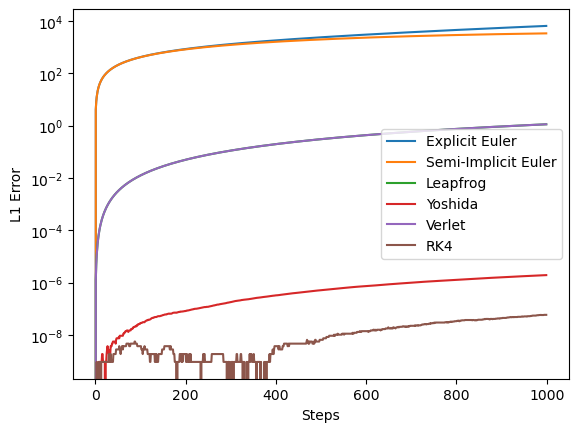
\includegraphics[scale=0.75]{Integration_comparison}
\caption{L1 Error plot of various physics integrators. Where the x-axis is the l1 error and the y-axis is the number of time steps taken. The l1 error was calculated with regards to the physics of a point mass with a circular orbit around another, fixed, point mass of greater mass. It was measured by $|r-r_t|$ where $r_t$ is the target radius and $r$ is the radius at step $t$.}
\end{figure}

\newpage

\bibliographystyle{acm}
\bibliography{References}

\end{document}